\subsection{Resumo da proposta}
	A proposta que será abordada pelo grupo é de coletar métricas referentes a custo, produtividade e usabilidade, melhorando a qualidade de desenvolvimento de software, com o propósito de agregar mais valor para a empresa.

\subsection{Lista de Software}
	Os softwares utilizados para o projeto serão os que já são utilizados na AEB, sendo eles: Gitlab e Gantt Project.Além desses, também será usado um editor de documentos para a criação dos questionários de satisfação; LaTeX; Google Drive; E Bizagi.

\subsection{Estrutura analítica do projeto - EAP}

\begin{figure}[H]
	\centering
	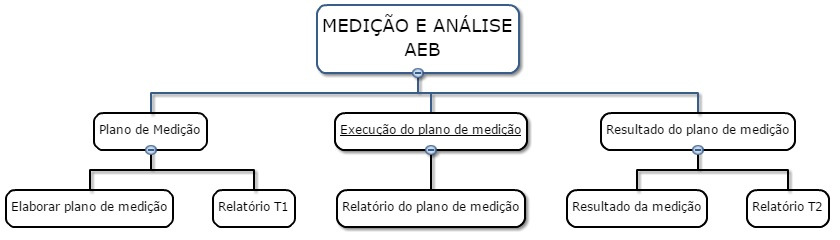
\includegraphics[width=\textwidth,height=\textheight,keepaspectratio]{conteudo/imgs/eap}
	\caption{Esstrutura Analítica do projeto - EAP}
	\label{img:eap}
\end{figure}

\subsection{Descrição de atividades}

\begin{figure}[H]
	\centering
	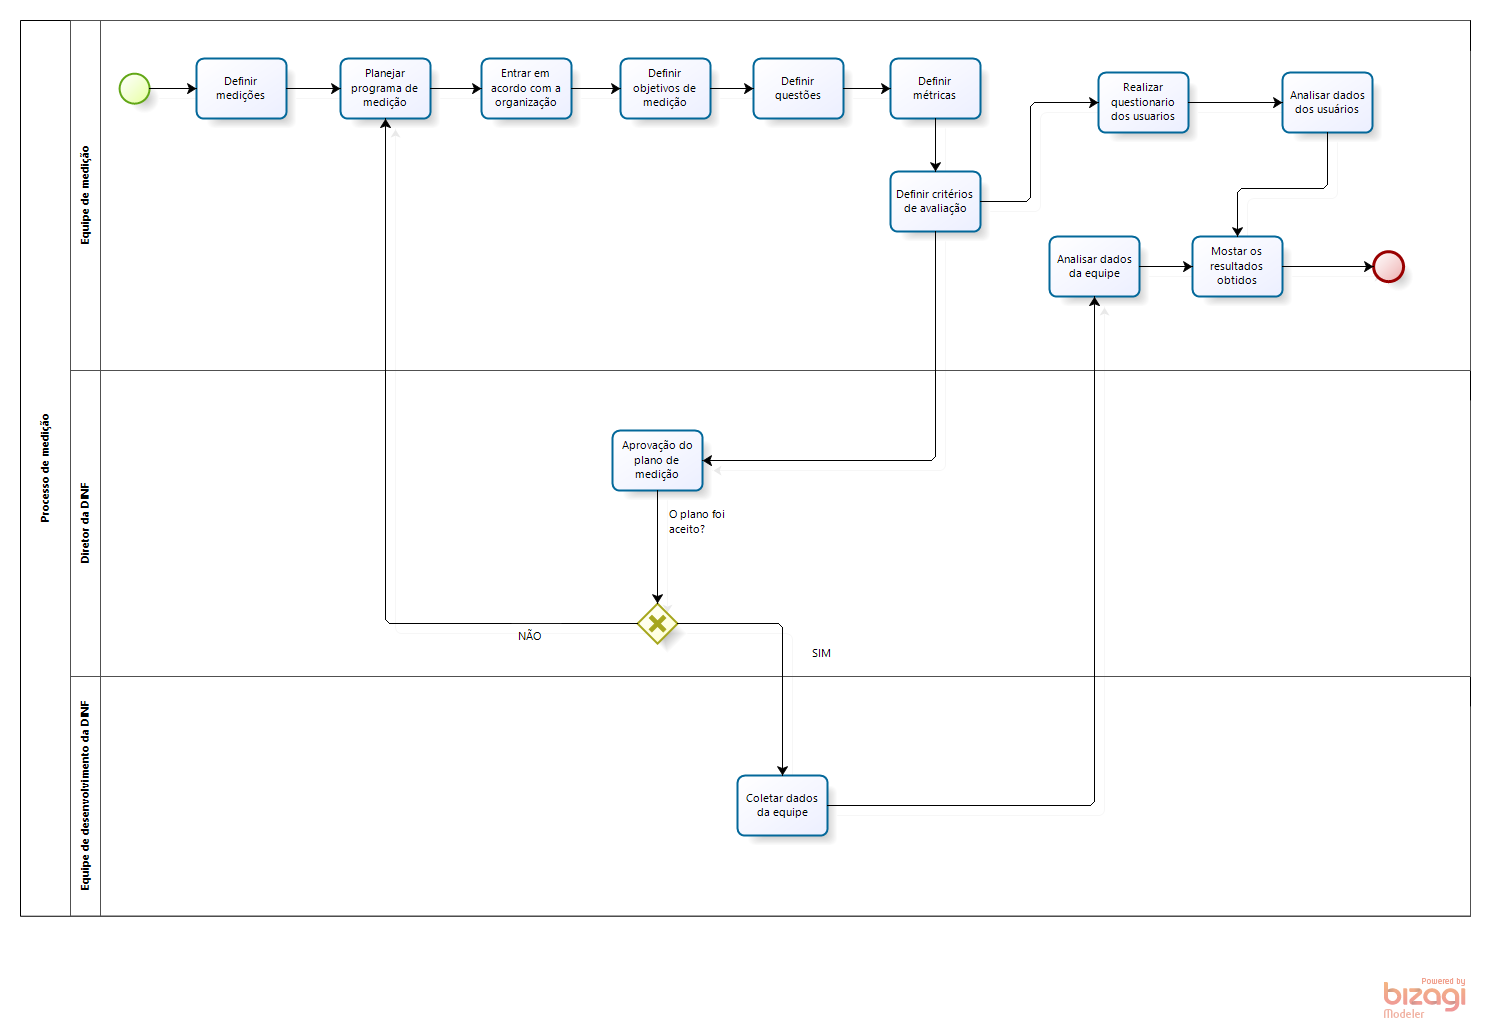
\includegraphics[width=\textwidth,height=\textheight,keepaspectratio]{conteudo/imgs/medicao}
	\caption{Modelagem do processo de medição}
	\label{img:modelagem1}
\end{figure}

\begin{table}[H]
\centering
\begin{tabular}{|p{1cm}|p{2cm}|p{5cm}|p{3cm}|}
\hline
	%-------------------------------------------------------
	\textbf{Id} &
	\textbf{Atividade} &
	\textbf{Descrição} &
  \textbf{Responsáveis}
	\\ \hline
	%-------------------------------------------------------
	A1 &
	Definir medições &
	Definir as medições de acordo com a organização &
	Time de medição e análise.
	\\ \hline
	%-------------------------------------------------------
	A2 &
	Planejar o programa de medições &
	Definir o programa de medição de acordo com a organização &
	Time de medição e análise.
	\\ \hline
	%-------------------------------------------------------
	A3 &
	Entrar em acordo com a organização &
	Definir juntamente com a organização as métricas a serem utilizadas no projeto &
	Time de medição e análise.
	\\ \hline
	%-------------------------------------------------------
	A4 &
	Aprovação do plano de medições &
	Versão estável do processo de medição &
	Time de medição e análise.
	\\ \hline

\end{tabular}
\caption{Fase 1. Entendimento do escopo do projeto}
\label{tab:atividades_fase_1}
\end{table}

\begin{table}[H]
\centering
\begin{tabular}{|p{1cm}|p{2cm}|p{5cm}|p{3cm}|}
\hline
	%-------------------------------------------------------
	\textbf{Id} &
	\textbf{Atividade} &
	\textbf{Descrição} &
  \textbf{Responsáveis}
	\\ \hline
	%-------------------------------------------------------
	A5 &
	Definir o objetivo de medição
 	Compreender quais são as necessidades da organização &
	Time de medição e análise.
	\\ \hline
	%-------------------------------------------------------
	A6 &
	Definir questões &
	Fazer uma caracterização do objeto de medição &
	Time de medição e análise.
	\\ \hline
	%-------------------------------------------------------
	A7 &
	Definir métricas &
	Definir métricas que serão usadas no processo da medição &
	Time de medição e análise
	\\ \hline
	%-------------------------------------------------------
	A8 &
	Definir critérios de avaliação &
	Escolher os critérios de avaliação baseado nas medições &
	Time de medição e análise.
	\\ \hline
\end{tabular}
\caption{Fase 2. Planejar processo de medição e análise}
\label{tab:atividades_fase_2}
\end{table}

\begin{table}[H]
\centering
\begin{tabular}{|p{1cm}|p{2cm}|p{5cm}|p{3cm}|}
\hline
	%-------------------------------------------------------
	\textbf{Id} &
	\textbf{Atividade} &
	\textbf{Descrição} &
  \textbf{Responsáveis}
	\\ \hline
	%-------------------------------------------------------
	A9 &
Coletar dados da equipe &
	Coletar medidas e medições a respeito da equipe de medição &
Time de medição e análise
	\\ \hline
	%-------------------------------------------------------
	A10 &
	Realizar questionários dos usuários &
Realizar questionários para saber a satisfação dos usuários do sistema &
Time de medição e análise.
		\\ \hline
\end{tabular}
\caption{Fase 3. Realizar medições}
\label{tab:atividades_fase_3}
\end{table}

\begin{table}[H]
\centering
\begin{tabular}{|p{1cm}|p{2cm}|p{5cm}|p{3cm}|}
\hline
	%-------------------------------------------------------
	\textbf{Id} &
	\textbf{Atividade} &
	\textbf{Descrição} &
  \textbf{Responsáveis}
	\\ \hline
	%-------------------------------------------------------
	A11 &
	Analisar dados da equipe de desenvolvimento &
	Formalizar as medidas coletadas da equipe de desenvolvimento &
Time de medição e análise.
	\\ \hline
	%-------------------------------------------------------
	A12 &
Analisar dados dos usuários &
  Formalizar as medidas coletadas através de questionários &
Time de medição e análise.
	\\ \hline
	%-------------------------------------------------------
	A13 &
Mostrar os resultados obtidos &
	Mostrar melhorias baseadas nas medições realizadas &
Time de medição e análise.
	\\ \hline
\end{tabular}
\caption{Fase 4. Resultados obtidos}
\label{tab:atividades_fase_4}
\end{table}

\subsection{Cronograma}

\begin{table}[H]
\centering
\begin{tabular}{|p{1cm}|p{2cm}|p{5cm}|p{3cm}|p{2cm}|p{2cm}|}
\hline
	%-------------------------------------------------------
	\textbf{Fase} &
	\textbf{ID} &
	\textbf{Atividade} &
	\textbf{Andamento} &
	\textbf{Deadline} &
	\textbf{Atribuição}
	\\ \hline

1 &
A1 &
Definir medições &
100\% &
09/09/16 &
Time de medição
\\ \hline
1 &
A2 &
Planejar o programa de medições &
100\% &
16/09/16 &
Time de medição
\\ \hline
1 &
A3 &
Entrar em acordo com a organização &
100\% &
16/09/16 &
Time de medição
\\ \hline
1 &
A4 &
Aprovação do plano de medições &
50\% &
26/09/16 &
Time de medição
\\ \hline
2 &
A5 &
Definir o objetivo de medição &
0\% &
07/10/16 &
Time de medição
\\ \hline
2 &
A6 &
Definir questões &
0\% &
07/10/16 &
Time de medição
\\ \hline
2 &
A7 &
Definir métricas &
0\% &
07/10/16 &
A definir
\\ \hline
2 &
A8 &
Definir critérios de avaliação &
0\% &
20/10/16 &
A definir
\\ \hline
3 &
A9 &
Coletar dados da equipe &
0\% &
20/10/16 &
A definir
\\ \hline
3 &
A10 &
Realizar questionários dos usuários &
0\% &
20/10/16 &
A definir
\\ \hline
4 &
A11 &
Analisar dados da equipe de desenvolvimento &
0\% &
20/10/16 &
A definir
\\ \hline
4 &
A12 &
Analisar dados dos usuários &
0\% &
11/11/16 &
A definir
\\ \hline
4 &
A13 &
Mostrar os resultados obtidos &
0\% &
11/11/16 &
A definir

	\\ \hline
\end{tabular}
\caption{Cronograma}
\label{tab:cronograma}
\end{table}
